%%KATRIN-Experiment.tex
%%

%% ==============
\chapter{Das KATRIN-Experiment}
\label{ch:Das KATRIN-Experiment}
%% ==============

Was macht Katrin, Neutrinomasse, unerreichte Senistivit�t usw.

\begin{figure}[ht]%
\centering
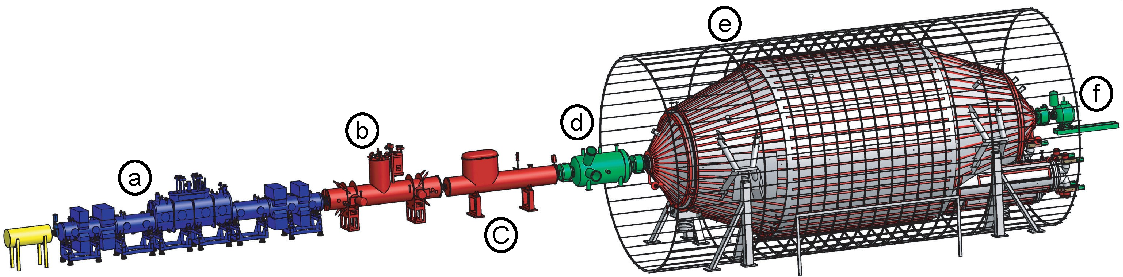
\includegraphics[width=\columnwidth]{Bilder/KATRIN/KATRIN_uebersicht.pdf}%
\caption[Aufbau des KATRIN-Experiments]{Der Aufbau des KATRIN-Experiments: Die fensterlose Quelle in blau (a), mit der Rear-Section in gelb, die differentielle (b) und kryogene (c) Pumpstrecke, das Vorspektrometer (d) sowie das Hauptspektrometer (e) mit seinen Luftspulensystemen und der Elektronendetektor (f) \cite{DTReich}}%
\label{fig:KATRIN_uebersicht}%
\end{figure}


%% ===========================

\section{Tritiumspektrum}
\section{MAC-E-Filter}
\section{Transmissionsfunktion}
\section{Aufbau von KATRIN}
\subsection{Fensterlose gasf�rmige Tritiumquelle}
\subsection{Spektrometer}
\subsection{Detektor}
%% ===========================

\section{Hochspannungslayout}

\dots
